
%(BEGIN_QUESTION)
% Copyright 2009, Tony R. Kuphaldt, released under the Creative Commons Attribution License (v 1.0)
% This means you may do almost anything with this work of mine, so long as you give me proper credit

Read and outline the ``Heat Transfer'' subsection of the ``Elementary Thermodynamics'' section of the ``Physics'' chapter in your {\it Lessons In Industrial Instrumentation} textbook.  Note the page numbers where important illustrations, photographs, equations, tables, and other relevant details are found.  Prepare to thoughtfully discuss with your instructor and classmates the concepts and examples explored in this reading.


\underbar{file i03978}
%(END_QUESTION)





%(BEGIN_ANSWER)

The following images were taken with an infra-red imaging camera, which shows the surface temperature(s) of an object by means of analyzing the infra-red light emitted by that object via {\it radiative} heat transfer.  It is interesting to note where each object is hottest, and to relate that to heat transfer not only with regard to the thermal images obtained but also to the regular thermodynamic behavior of that object.  Questions you may wish to pose include:

\begin{itemize}
\item{} Where is each object appear to be the hottest?  Why?
\item{} Where is each object appear to be the coldest?  Why?
\item{} How does each object shed heat during its ordinary day-to-day function?
\item{} Is there more than one mode of heat transfer at work here?
\end{itemize}






\vfil \eject

Heat transfer example -- infrared theral image of a Jeep vehicle after being driven:

$$\epsfxsize=6in \includegraphics[width=15.5cm]{i03978x01.eps}$$

Internal combustion engines are {\it heat engines}, developing mechanical power by heating a gas (air) to high temperatures and forcing the resulting expansion of that gas to press against a surface (called a {\it piston}) to do useful work.  In the process, a lot of ``waste'' heat is created, which the engine must shed or else suffer damage from overheating.

This is why engines have {\it radiators}: to shed the excess heat energy to the surrounding environment.  Can you see where the radiator is in this thermal image?








\vfil \eject

Heat transfer example -- infrared theral image of a chest freezer as it is running:

$$\epsfxsize=5in \includegraphics[width=15.5cm]{i03978x02.eps}$$

Refrigerators and freezers do not magically ``make cold,'' but rather force heat transfer to occur where it usually would not.  Recall that heat spontaneously flows from areas of high temperature to areas of low temperature.  This means a refrigeration unit must somehow force heat to flow ``backwards'' from a cold area to a warmer area.  In a compressed-gas refrigerator unit, this happens because a compressor compresses a gas to a high pressure (which also causes that gas to rise in temperature), then sends that gas through a series of tubes called a {\it condensor} where the hot gas naturally loses heat energy to the (cooler) outside air.  After losing heat, this high-pressure gas condenses into a high-pressure liquid.  This liquid is then sent to another series of tubes called an {\it evaporator} where the liquid experiences a sharp drop in pressure and re-boils into a gas.  This change of phase from liquid to gas requires an input of thermal energy, which takes the form of the boiling liquid (and boiled vapor) becoming much colder.  

Thus, heat flows naturally as it always does from a warmer area to a colder area at both the condensor and the evaporator.  At the condensor, hot gas loses heat to the outside air and condenses into liquid at the same time.  At the evaporator, cold liquid gains heat from the inside of the refrigerator/freezer unit and boils into gas at the same time.  The ``magic'' of a refrigeration unit is that heat energy is carried from the cold evaporator to the hot condensor by the working fluid when forced to flow that way by the compressor.

\vskip 10pt

The condensor may be seen in this thermal image as a series of lines along the side of the freezer unit, giving off heat to the surrounding air.  The evaporator lies just underneath the inside walls of the freezer, absorbing heat from the interior of the freezer to make that space cold.







\vfil \eject

Heat transfer example -- infrared theral image of a parrot:

$$\epsfxsize=6in \includegraphics[width=15.5cm]{i03978x03.eps}$$

All animals live by metabolizing food.  This is essentially a slow, low-temperature form of {\it combustion}, where carbohydrate and fat molecules (primarily) in the food combine with oxygen to form carbon dioxide gas and heat.  Like the internal combustion engine in a vehicle, there is a lot of ``waste'' heat generated in this process, which must be shed lest the animal overheat.  

Here, you can see areas on the parrot's skin that appear warm.  Most of the parrot's body, however, appears much colder because it is insulated by a thick layer of feathers.  This is the primary function of feathers: to provide thermal insulation.  This is why even flightless birds (such as penguins) have feathers.

\vskip 10pt

Can you see an area on this bird's perch that has become warmer due to contact with the bird's feet?  What form of heat transfer is this?











\vfil \eject

Heat transfer example -- infrared theral image of the author wearing a hat:

$$\epsfxsize=6in \includegraphics[width=15.5cm]{i03978x04.eps}$$

Here we see a thermal image of the author, showing just how hot his head is.  This explains a lot, perhaps more than the author is prepared to admit.

Compare the surface temperature of this person against the surface temperature of the parrot.  Why do the two bodies appear so different?

\vskip 10pt

An interesting artifact of infra-red thermal imaging is apparent in this image: note how the eyeglass lenses appear cold (blue).  Most glasses and plastic materials are opaque to infra-red light, which means the author's warm eyes are invisible to the infra-red camera so long as he is wearing his glasses.








%(END_ANSWER)





%(BEGIN_NOTES)

Three modes of heat transfer exist:

\begin{itemize}
\item{} Radiation (light waves emitted from hot objects)
\item{} Conduction (direct contact between objects)
\item{} Convection (intermediate contact using a heat-transfer fluid)
\end{itemize}

Optical pyrometers use radiative heat transfer to sense temperature.  Direct-contact thermocouples use conductive heat transfer to sense temperature.  A sensor in a fluid-filled pipe use convective heat transfer to sense temperature.

\vskip 10pt

Radiation is the least efficient means of heat transfer:

$${dQ \over dt} = e \sigma A T^4$$

\noindent
Where,

$dQ \over dt$ = Radiant heat loss rate (watts)

$e$ = Emissivity factor (unitless)

$\sigma$ = Stefan-Boltzmann constant (5.67 $\times$ $10^{-8}$ W / m$^{2}$ $\cdot$ K$^{4}$)

$A$ = Surface area (square meters)

$T$ = Absolute temperature (Kelvin)

\vskip 10pt

Emissivity varies with color and texture.  Dark and rough surfaces have high emissivity, while light and smooth surfaces have low emissivity.  Radiation is bi-directional, with high-emissivity objects being both good collectors and radiators of thermal energy.

\vskip 10pt

Conduction of heat is proportional to the surface area of mutual contact and the difference of temperature across that contact area.  Conduction is inversely proportional to the length that the heat must travel through:

$${dQ \over dt} = {kA {\Delta T} \over l}$$

\noindent
Where,

$dQ \over dt$ = Conductive heat transfer rate

$k$ = Thermal conductivity 

$A$ = Surface area 

$\Delta T$ = Difference of temperature between ``hot'' and ``cold'' sides

$l$ = Length of heat flow path from ``hot'' to ``cold'' side

\vskip 10pt

``R-value'' is an expression of thermal insulation, with a greater R value representing less conductivity to heat transfer, equivalent to $l \over k$ when British units are used.

\vskip 10pt

Convection is where fluid molecules alternately absorb heat from a hot object then release heat to a cold object, serving as a medium for heat transfer between two objects.  {\it Heat exchangers} are special devices built to transfer heat between two different fluids.  Heat exchangers find common use in the process industries, to transfer energy between fluids for processing needs and energy conservation needs.

A {\it thermosiphon} is a self-pumping loop of fluid motivated by a difference in temperature.  Heated fluid becomes less dense and rises, while cooled fluid becomes denser and sinks.  Thus a ``natural convection'' takes place if the fluid loop has any substantial vertical span.





\vskip 20pt \vbox{\hrule \hbox{\strut \vrule{} {\bf Suggestions for Socratic discussion} \vrule} \hrule}

\begin{itemize}
\item{} Describe the purpose and construction of a {\it heat exchanger}, as well as some practical examples in industry.
\item{} If one desired to minimize an object's radiative heat loss, how could that object be modified to achieve this end?  A good example of this is a space station, where radiation is the primary means of heat transfer from the station to the empty vacuum of space surrounding it.
\item{} If one desired to minimize an object's conductive heat loss, how could that object be modified to achieve this end?  A good example of this is a hot frying pan which you intend to set on a cold counter-top, but desire to avoid having that pan scorch the counter-top.
\item{} If one desired to minimize an object's convective heat loss, how could that object be modified to achieve this end?  A good example of this is keeping a warm cup of coffee from cooling off too fast when carried outside on a cold, windy day.
\item{} Examine the simple P\&IDs shown in this section of the textbook, and explain how heat exchangers perform a useful function in those processes.
\end{itemize}












\vfil \eject

\noindent
{\bf Prep Quiz:}

A woman stands far away from a roaring campfire, yet feels the heat of the fire against her face.  This is an example of which type of heat transfer method?

\begin{itemize}
\item{} Convection
\vskip 5pt 
\item{} Conduction
\vskip 5pt 
\item{} Turbulence
\vskip 5pt 
\item{} Bimetallic
\vskip 5pt 
\item{} Filled-system
\vskip 5pt 
\item{} Radiation
\end{itemize}









\vfil \eject

\noindent
{\bf Prep Quiz:}

A boy accepts a dare to touch the hot burner of a kitchen stove, and burns his hand in the process.  This is an example of which type of heat transfer method?

\begin{itemize}
\item{} Convection
\vskip 5pt 
\item{} Conduction
\vskip 5pt 
\item{} Turbulence
\vskip 5pt 
\item{} Bimetallic
\vskip 5pt 
\item{} Idiotic
\vskip 5pt 
\item{} Radiation
\end{itemize}








\vfil \eject

\noindent
{\bf Prep Quiz:}

A man standing outside on a cold day warms his hands by blowing air into them from his mouth, transferring heat from deep inside his body.  This is an example of which type of heat transfer method?

\begin{itemize}
\item{} Convection
\vskip 5pt 
\item{} Conduction
\vskip 5pt 
\item{} Turbulence
\vskip 5pt 
\item{} Bimetallic
\vskip 5pt 
\item{} Filled-system
\vskip 5pt 
\item{} Radiation
\end{itemize}

%INDEX% Reading assignment: Lessons In Industrial Instrumentation, Elementary Thermodynamics (heat and transfer)

%(END_NOTES)


